\RequirePackage{fix-cm}
\documentclass[twocolumn]{svjour3}

\usepackage{cite}
\usepackage{graphicx}
\usepackage{amsmath}
\usepackage{amsfonts}
\usepackage{amssymb}
\usepackage{xcolor}
\usepackage{mathtools}
\usepackage{bm}
\usepackage{upgreek}
\usepackage{adjustbox}
\usepackage{placeins}    
\usepackage{balance}
\usepackage[misc]{ifsym}
\usepackage{url}
\usepackage{multirow}
\usepackage{tikz}
\usepackage{soul}

\newcommand\hhl[1]{%
	\bgroup
	\hskip0pt\color{blue!80!blue}%
	#1%
	\egroup
}

%%%%%%%%%%%%%%%%%%%%%%%%%%%

\journalname{Nonlinear Dynamics}
	
\begin{document}
	
	\title{\hl{Nie uzupelniac}}
	
	\titlerunning{\hl{Nie uzupelniac}}
	
	\author{Adam~Soko{\l}owski, Robert~Nebeluk}
	
	\authorrunning{A.~Soko{\l}owski, R.~Nebeluk} 
	
	\institute{A.~Soko{\l}owski, R.~Nebeluk, \at
		Warsaw University of Technology\\
		Institute of Control and Computation Engineering\\  
		ul. Nowowiejska 15/19, 00-665 Warsaw, Poland\\
		\email{ \hl{a.sokolowski2003@gmail.com}, Robert.Nebeluk@pw.edu.pl}
	}
	
	\date{Received: date / Accepted: date}
	% The correct dates will be entered by the editor

	\maketitle
	
	\begin{abstract}
		\hl{Nie uzupelniac}
		\keywords{\hl{Nie uzupelniac}}
	
	\end{abstract}
	
	\section{Introduction}
	\label{sec:p}
    \hl{Nie uzupelniac}\\
    \hl{Na wszelki wypadek: prosze pamietac aby nie generowac tekstu przy pomocy narzedzi AI - pliki zrodlowe po wyslaniu beda sprawdzane przez odpowiednie narzedzia. Dopoki sam Pan tlumaczy i sam Pan wymysla kolejne linijki tekstu to na pewno bedzie wszystko w porzadku.}
    \section{Modeling of inverted pendulum on cart system}
	\label{sec:pp}
\begin{figure}[!htbp]
\centering
\includegraphics[scale=0.35]{Img/model.png}
\caption{Schematic of the inverted pendulum on a cart~\cite{Prasad2014}. Indicated are the cart position $x_\mathrm{p}(t)$ (measurement point $x_{\mathrm{p}1}$), pendulum angle $\theta(t)$, horizontal control force $F(t)$, and bidirectional external disturbance $F_\mathrm{w}(t)$.}
\label{fig:model}
\end{figure}
\hl{TODO later: Update Fig. 1 (draw.io): replace u with F, x with x\_p1; do not introduce y\_p1 (always zero on the track); mark F\_w with a bidirectional arrow and a dimension line for l sin theta; remove the dashed line under the wheels; set all figure labels in math mode.}

The inverted pendulum on a cart is a well-known underactuated mechanical system and a widely
used benchmark for testing control algorithms~\cite{Prasad2014}. It consists of a
cart of mass $M$ that moves along a horizontal track, with a pendulum of mass $m$ and length
$l$ attached to it by a frictionless pivot. In the physical model the only control input is the
horizontal force $F(t)$ applied to the cart; an external disturbance $F_\mathrm{w}(t)$ acting
horizontally on the pendulum tip is also considered. The symbols $u$ and $y$ are reserved for
the discrete-time control signal and the controlled output in the closed-loop study
(Section~\ref{sec:r}). The physical parameters used in this work are listed in
Table~\ref{tab:params}.
\hl{TO DO: Prosze zaznaczyc na rysunku $F_\mathrm{w}$, jesli sila dziala w lewo i w prawo to strzalka dwukierunkowa; jezeli odl. $l\sin\theta$ jest pomiedzy (tam gdzie jest teraz napisane) to poprowadzic linie laczaca od grotu lewej do grotu prawej strzalki, symbole zapisac wszystkie na rysunku w trybie matematycznym (jesli jest to w drawio to: https://www.drawio.com/docs/manual/text/math-typesetting/)}
\setlength\tabcolsep{4pt}
\begin{table}[htbp]
\caption{Physical parameters of the inverted-pendulum system.}
\label{tab:params}
\centering
\begin{small}
\begin{tabular}{lcc}
\hline
\rule{0pt}{3mm}Parameter & Symbol & Value \\
\hline
\rule{0pt}{3.5mm}Cart mass         & $M$ & $2.40$~kg \\
Pendulum mass     & $m$ & $0.23$~kg \\
Pendulum length   & $l$ & $0.36$~m  \\
Gravitational acceleration & $g$ & $\phantom{000} 9.81$~m/s$^{2}$ \\
\hline
\end{tabular}
\end{small}
\end{table}

The following simplifying assumptions are made~\cite{Prasad2014}: the rod is massless and
rigid; friction at the wheels and at the pivot is negligible; motion is planar; and the
pendulum mass is treated as a point mass at the rod tip. The angle $\theta(t)$ measures the
pendulum deflection from the upright position (positive clockwise, $\theta=0$ at the top),
and $x_\mathrm{p}(t)$ is the cart position along the track. Because the cart is constrained to
the horizontal axis, its vertical coordinate is identically zero and is not introduced.

\subsection{Equations of motion}
In this modelling section the cart force is denoted $F(t)$. In the controllers of
Section~\ref{sec:r} the same physical force sampled at $t=kT_p$ is written as the control
signal $u(k)=F(kT_p)$, while the controlled output $y$ is taken as $\theta$ or $x_\mathrm{p}$,
depending on the indicator.

Following~\cite{Prasad2014}, the position of the pendulum tip (centre of gravity) in the fixed frame is
\begin{equation}
x_\mathrm{G}(t) = x_\mathrm{p}(t) + l\sin\theta(t),\qquad
y_\mathrm{G}(t) = l\cos\theta(t).
\label{eq:cog}
\end{equation}
Differentiating \eqref{eq:cog} twice with respect to time yields the tip accelerations
\begin{align}
\ddot{x}_\mathrm{G}(t)
&= \ddot{x}_\mathrm{p}(t) + l\cos\theta(t)\,\ddot{\theta}(t)
 - l\sin\theta(t)\,\dot{\theta}^{2}(t),
\label{eq:acc_xg}\\
\ddot{y}_\mathrm{G}(t)
&= -l\sin\theta(t)\,\ddot{\theta}(t)
 - l\cos\theta(t)\,\dot{\theta}^{2}(t).
\label{eq:acc_yg}
\end{align}
Newton's second law for the complete system in the horizontal direction,
$M\ddot{x}_\mathrm{p}+m\ddot{x}_\mathrm{G}=F+F_\mathrm{w}$, together with \eqref{eq:acc_xg}, gives the translational equation~\cite{Prasad2014}:
\begin{multline}
(M{+}m)\ddot{x}_\mathrm{p}(t) + ml\cos\theta(t)\,\ddot{\theta}(t) \\
- ml\sin\theta(t)\,\dot{\theta}^{2}(t) = F(t) + F_\mathrm{w}(t).
\label{eq:trans}
\end{multline}

A torque balance about the pivot is obtained from the inertial force components
$F_x=m\ddot{x}_\mathrm{G}$ and $F_y=m\ddot{y}_\mathrm{G}$ acting at the tip,
together with gravity and the disturbance moment $(F_\mathrm{w}\cos\theta)\,l$~\cite{Prasad2014}:
\begin{equation}
\bigl(F_x\cos\theta(t)\bigr)l - \bigl(F_y\sin\theta(t)\bigr)l
= \bigl(mg\sin\theta(t)\bigr)l + \bigl(F_\mathrm{w}(t)\cos\theta(t)\bigr)l.
\label{eq:torque_raw}
\end{equation}
Substituting \eqref{eq:acc_xg}--\eqref{eq:acc_yg} into \eqref{eq:torque_raw} and simplifying
($\cos^{2}\theta+\sin^{2}\theta=1$) yields the rotational equation
\begin{multline}
ml\cos\theta(t)\,\ddot{x}_\mathrm{p}(t) + ml^{2}\ddot{\theta}(t) \\
= mgl\sin\theta(t) + lF_\mathrm{w}(t)\cos\theta(t).
\label{eq:rot}
\end{multline}
The auxiliary quantities
\begin{equation}
M_T = M+m,
\label{eq:MT}
\end{equation}
\begin{equation}
D(t)=l\bigl(M_T - m\cos^{2}\!\theta(t)\bigr)
\label{eq:Dt}
\end{equation}
are introduced next. Solving \eqref{eq:trans}--\eqref{eq:rot} for the cart acceleration
first gives~\cite{Prasad2014}
\begin{equation}
\ddot{x}_\mathrm{p}(t) =
\frac{F(t) + ml\sin\theta(t)\,\dot{\theta}^{2}(t)
 - mg\sin\theta(t)\cos\theta(t)
 + F_\mathrm{w}(t)\sin^{2}\theta(t)}{M_T - m\cos^{2}\!\theta(t)}.
\label{eq:xdd}
\end{equation}

Substituting \eqref{eq:xdd} back into \eqref{eq:rot} (or applying the same algebraic elimination
to the angular acceleration) then yields
\begin{equation}
\ddot{\theta}(t) =
\frac{M_T g\sin\theta(t)
 - \cos\theta(t)\!\left(F(t) + ml\sin\theta(t)\,\dot{\theta}^{2}(t)\right)
 + \dfrac{M}{m}F_\mathrm{w}(t)\cos\theta(t)}{D(t)}.
\label{eq:tdd}
\end{equation}
\subsection{Nonlinear state-space model}

Defining the state vector
\begin{equation}
    x(t) = \bigl[\theta(t),\,\dot{\theta}(t),\,x_\mathrm{p}(t),\,\dot{x}_\mathrm{p}(t)\bigr]^T,
\end{equation}
the dynamics \eqref{eq:xdd}--\eqref{eq:tdd} take the form
\begin{equation}
    \dot{x}(t) = f\bigl(x(t),F(t),F_\mathrm{w}(t)\bigr):
\end{equation}
\begin{equation}
\resizebox{\columnwidth}{!}{$\displaystyle
\begin{bmatrix}\dot{x}_1(t)\\\dot{x}_2(t)\\\dot{x}_3(t)\\\dot{x}_4(t)\end{bmatrix}
=
\begin{bmatrix}
x_2(t)\\[2pt]
\dfrac{M_T g\sin x_1(t) - \cos x_1(t)\!\left(F(t) + ml\sin x_1(t)\,x_2^{2}(t)\right)
 + \frac{M}{m}F_\mathrm{w}(t)\cos x_1(t)}{D(t)}\\[6pt]
x_4(t)\\[2pt]
\dfrac{F(t) + ml\sin x_1(t)\,x_2^{2}(t) - mg\sin x_1(t)\cos x_1(t)
 + F_\mathrm{w}(t)\sin^{2}x_1(t)}{M_T - m\cos^{2}\!x_1(t)}
\end{bmatrix}$}.\label{eq:nonlin_ss}
\end{equation}

\subsection{Linearized model}
The system \eqref{eq:nonlin_ss} has $n=4$ state variables, one control input, and one
disturbance input.
For small deflections around the upright equilibrium ($\theta\approx 0$), the approximations
$\sin\theta\approx\theta$, $\cos\theta\approx 1$ yield the linear time-invariant
state-space model~\cite{Prasad2014}:
\begin{equation}
\dot{x}(t) = Ax(t) + BF(t) + B_\mathrm{d}F_\mathrm{w}(t),
\label{eq:linsys}
\end{equation}
where $A\in\mathbb{R}^{n\times n}$ is the system matrix, $B\in\mathbb{R}^{n\times 1}$ is the
control input matrix, and $B_\mathrm{d}\in\mathbb{R}^{n\times 1}$ is the disturbance input
matrix:
\begin{equation}
A = \begin{bmatrix}0&1&0&0\\ \dfrac{M_T g}{Ml}&0&0&0\\[4pt]0&0&0&1\\[2pt]-\dfrac{mg}{M}&0&0&0\end{bmatrix},\;
B = \begin{bmatrix}0\\[2pt]-\dfrac{1}{Ml}\\[4pt]0\\[2pt]\dfrac{1}{M}\end{bmatrix},\;
B_\mathrm{d} = \begin{bmatrix}0\\[2pt]-\dfrac{1}{ml}\\[4pt]0\\[2pt]0\end{bmatrix}.
\label{eq:linear}
\end{equation}
The eigenvalues of $A$ are found from the characteristic equation $\det(\lambda I - A)=0$,
which for the given parameter values yields:
\begin{equation}
\lambda^4 - \frac{(M+m)g}{Ml}\,\lambda^2 = 0.
\label{eq:charpoly}
\end{equation}
Solving \eqref{eq:charpoly} gives four eigenvalues:
$\lambda_{1,2}=0$ and $\lambda_{3,4}=\pm\sqrt{\tfrac{(M+m)g}{Ml}}\approx\pm 5.49$.
The positive eigenvalue $\lambda_4>0$ confirms that the system is open-loop unstable.
The controllability matrix $\mathcal{C}=[B,\;AB,\;A^2B,\;A^3B]\in\mathbb{R}^{n\times n}$
satisfies $\mathrm{rank}(\mathcal{C})=n=4$, so a stabilising feedback law exists.
    \section{Control system design}
	\label{sec:r}
    The shared discrete-time state vector is:
\begin{equation}
x(k)=\bigl[\theta(k),\;\dot{\theta}(k),\;x_\mathrm{p}(k),\;\dot{x}_\mathrm{p}(k)\bigr]^T,
\label{eq:state_vec}
\end{equation}
where the components are the pendulum angle, angular velocity, cart position, and cart
velocity, respectively. The control signal $u(k)$ equals the cart force at the sampling
instant, $u(k)=F(kT_p)$. The controlled output used later for quality assessment is denoted
$y$ and is either $\theta$ or $x_\mathrm{p}$. All controllers work in discrete time with
sampling period $T_p$.

\subsection{PID control scheme}
The parallel PID structure~\cite{Prasad2014} uses two independent PID loops whose outputs are
added together:
\begin{equation}
u(k) = u_{\theta}(k) + u_{x}(k),
\end{equation}
where the tracking errors are defined as:
\begin{align}
e_{\theta}(k) &= \theta_\mathrm{ref} - x_1(k), \label{eq:err_theta}\\
e_x(k) &= x_\mathrm{ref} - x_3(k). \label{eq:err_x}
\end{align}
Here $\theta_\mathrm{ref}=0$ is the desired upright angle and $x_\mathrm{ref}$ is the desired
cart position $x_\mathrm{p}$.
Each loop uses a discrete-time PID law with \emph{derivative on measurement}, which avoids
amplifying measurement noise:
\begin{align}
u_{\theta}(k) &= K_{p,\theta}e_{\theta}(k) + K_{i,\theta}\!\sum_{j=0}^{k}\!e_{\theta}(j)T_p
               - K_{d,\theta}x_2(k),\label{eq:pid_theta}\\
u_{x}(k) &= K_{p,x}e_x(k) + K_{i,x}\!\sum_{j=0}^{k}\!e_x(j)T_p
           - K_{d,x}x_4(k).\label{eq:pid_x}
\end{align}
where $K_{p,\cdot}$, $K_{i,\cdot}$, $K_{d,\cdot}$ are the proportional, integral, and
derivative gains for the angle and position loops, respectively. The velocity states
$x_2(k)$ and $x_4(k)$ are used in place of the numerical error derivative
(derivative-on-measurement technique), eliminating the derivative kick at reference steps.
An anti-windup mechanism limits the integral accumulation. The clamped integral state obeys:
\begin{equation}
I_{\theta}(k) = \mathrm{sat}\!\left(I_{\theta}(k{-}1)+e_{\theta}(k)T_p,\;-I_{\max},\;I_{\max}\right),
\label{eq:antiwindup}
\end{equation}
where $\mathrm{sat}(\cdot,\,a,\,b)=\max\!\bigl(a,\min(b,\cdot)\bigr)$ is the saturation
function and $I_{\max}=5.0$. The same clamping applies to the position-loop integral
$I_x(k)$.

\subsection{LQR control scheme}
The Discrete Linear Quadratic Regulator (DLQR)~\cite{Jezierski2017} computes a
state-feedback gain $K$ that minimises the infinite-horizon cost:
\begin{equation}
J = \sum_{k=0}^{\infty}\!\left(x(k)^T Q\,x(k) + u(k)^T R\,u(k)\right),
\label{eq:lqr_cost}
\end{equation}
where $Q\in\mathbb{R}^{n\times n}$, $Q\succeq 0$ is the state weighting matrix and
$R\in\mathbb{R}^{1\times 1}$, $R>0$ is the control weighting matrix,
subject to the linearised discrete model $x(k{+}1)=A_dx(k)+B_du(k)$,
where $A_d\in\mathbb{R}^{n\times n}$, $B_d\in\mathbb{R}^{n\times 1}$ are obtained from
$(A,B)$ of \eqref{eq:linear} via zero-order-hold (ZOH)
discretisation at period $T_p$. The optimal gain is found from the positive-definite solution $P\in\mathbb{R}^{n\times n}$ of the Discrete Algebraic
Riccati Equation (DARE):
\begin{equation}
P = A_d^T P A_d - A_d^T P B_d(R+B_d^T P B_d)^{-1}B_d^T P A_d + Q,
\end{equation}
yielding:
\begin{equation}
K = (R + B_d^T P B_d)^{-1}B_d^T P A_d,
\end{equation}
where $K\in\mathbb{R}^{1\times n}$ is the optimal state-feedback gain vector, and the control
law is $u(k) = -K\bigl(x(k) - x_\mathrm{ref}\bigr)$.

\subsection{LQR-I control scheme}

To eliminate steady-state cart-position error, the DLQR is augmented with an integrator
acting on the position tracking error. The accumulated error state is:
\begin{equation}
z(k+1) = z(k) + \bigl(x_\mathrm{ref} - x_3(k)\bigr)T_p.
\end{equation}
The augmented state $x_\mathrm{aug}(k)=[x_1,x_2,x_3,x_4,z]^T\in\mathbb{R}^{n+1}$ obeys:
\begin{equation}
x_\mathrm{aug}(k{+}1) = \tilde{A}_d\,x_\mathrm{aug}(k) + \tilde{B}_d\,u(k),
\end{equation}
where $\tilde{A}_d\in\mathbb{R}^{5\times 5}$ and $\tilde{B}_d\in\mathbb{R}^{5\times 1}$
append the integrator row to $A_d$ and $B_d$, respectively. Applying DLQR to the augmented
system with extended weighting matrices $\tilde{Q}\in\mathbb{R}^{(n+1)\times(n+1)}$ and $R$ yields:
\begin{equation}
u(k) = -\tilde{K}\,x_\mathrm{aug}(k),
\end{equation}
which gives zero steady-state position error for constant setpoints.

\subsection{PID-LQR control scheme}

The PID-LQR scheme~\cite{Prasad2014,Nguyen2024} combines DLQR stabilisation with an outer PID loop on the position
error:
\begin{equation}
u(k) = u_\mathrm{LQR}(k) + u_\mathrm{PID,pos}(k),
\end{equation}
where the LQR component acts on the full state:
\begin{equation}
u_\mathrm{LQR}(k) = -K\bigl(x(k) - x_\mathrm{ref}\bigr),
\end{equation}
and $u_\mathrm{PID,pos}(k)$ follows the discrete PID law of \eqref{eq:pid_x} acting only on the
cart-position loop. This structure improves setpoint tracking and reduces steady-state errors
caused by model mismatch.

\subsection{Fuzzy LQR control scheme}

In Fuzzy-LQR~\cite{Nguyen2024}, a Takagi-Sugeno (T-S) fuzzy block runs in parallel with the DLQR:
\begin{equation}
u(k) = u_\mathrm{LQR}(k) + G\cdot u_\mathrm{Fuzzy}(k).
\end{equation}
Triangular membership functions over two linguistic sets (\emph{small error},
\emph{large error}) for each of the four state variables yield a rule base of
$2^4=16$ rules of the form:
\begin{quote}
\textbf{IF} $e_\theta$ is $A_i$ \textbf{AND} $\dot\theta$ is $B_i$
$\ldots$ \textbf{THEN} $u_i = -K^{(i)}x$.
\end{quote}
The local gain vectors adapt to the severity of the deviation:
\begin{equation}
K^{(i)} = K_\mathrm{base} + \alpha\,L_i,
\end{equation}
where $L_i\in\{0,\ldots,4\}$ counts how many state variables are currently in the
\emph{large-error} region, and $\alpha$ is a fixed step. The defuzzified output is the
weighted average:
\begin{equation}
u_\mathrm{Fuzzy}(k) = \frac{\displaystyle\sum_{i=1}^{16}w_i(x)\,u_i}
                           {\displaystyle\sum_{i=1}^{16}w_i(x)},
\end{equation}
where $w_i$ is the firing strength of rule $i$ and $G$ is a global scaling gain. As a result,
the controller reacts more strongly at large deflections and more gently near the equilibrium.

\subsection{MPC-NO control scheme}

At each sampling instant the Nonlinear MPC (NMPC)~\cite{Mills2009} solves the following
finite-horizon optimisation problem:
\begin{multline}
\min_{\Delta u(k)}\;J(k) = \sum_{p=1}^{N}e_p(k)^T Q\,e_p(k) \\
+ \sum_{p=0}^{N_u-1}\Delta u_p(k)^T R\,\Delta u_p(k),
\label{eq:mpc_cost}
\end{multline}
where the predicted state error vector $e_p(k)\in\mathbb{R}^{n}$ and the control increment
$\Delta u_p(k)\in\mathbb{R}$ are defined as:
\begin{align}
e_p(k) &= x_\mathrm{ref}(k{+}p|k) - \hat{x}(k{+}p|k), \label{eq:ep}\\
\Delta u_p(k) &= u(k{+}p|k) - u(k{+}p{-}1|k), \label{eq:dup}
\end{align}
$Q\in\mathbb{R}^{n\times n}$, $Q\succeq 0$ is the state weighting matrix,
$R>0$ is the control weighting scalar, $N$ is the prediction
horizon, and $N_u\leq N$ the control horizon, subject to:
\begin{align}
\hat{x}(k+1) &= f\!\left(\hat{x}(k),u(k)\right),\quad k=0,\ldots,N{-}1,\\
u_{\min} &\leq u(k) \leq u_{\max}.
\end{align}
The prediction model $f(\cdot)$ propagates the nonlinear dynamics \eqref{eq:nonlin_ss} over
one sampling period using fourth-order Runge-Kutta (RK4), with $u(k)$ identified with $F(kT_p)$
and held constant within each interval (ZOH). The optimisation is solved by the SLSQP algorithm from
\texttt{scipy.optimize}.

\subsection{MPC-NO-alt control scheme}
\hl{Czy w literaturze [1] bylo pokazane odwrocena wahadlo na wozku i rozwazana taka postac funkcji kosztu? Jesli tak to o tym powiedziec, jezeli nie i po prostu bylo pokazane, ze ogolnie mozna taki koszt zastosowac to tak jeszcze skomentowac. Potrzebna bedzie literatura zwiazana z funkcjami kosztu w MPC, ktore byly stosowane dla tego konkretnie obiektu. Prosilbym Pana o poszukanie, zapewne znajdzie Pan w wiekszosci klasyczna funkcje kosztu L2 (dwa, nie trzy, człony w J(k)) ale prosze takie artykuly tez zachowac. Najwazniejsze tu jest dotrzec do tych mniej uzywanych, jakichs alternatywnych kosztow. Drugi "problem": prosze rozgladac sie rowniez za literatura ktora mowi o zaletach/korzysciach z stosowania wlasnie takich czlonow jak Pan zostosowal w kontekscie wahadla, czyli czlonow z kara na wart. sterowania lub/i przyrost. Trzeba uargumentowac dlaczego jest to potrzebne dla tego przykladu, co chcemy tym uzyskac, moze Pan znajdzie literature gdzie byly badania robione (nie jedne) ktore dla tego przykladu mowia o istotnosci tych czlonow, zapewne Pan je odrozni, bo bedzie pokazane dosc dokladnie strojenie regulatorow. Zaznaczam, ze literatury trzeba do art. szukac jak najwiecej, zwlaszcza, ze jest to obiekt bardzo znany, wiec recenzenci to zauwaza. Moze Pan jednym zdaniem kazda literature skomentowac we wstepie, potem zastanowimy sie, ulozy sie i wklei do odpowiedniej sekcji}
For the cart--pendulum, the classical two-term quadratic cost (tracking error + control effort)
is the default choice in NMPC studies such as~\cite{Mills2009}. The textbook formulation
of~\cite{Camacho2007} already admits move-suppression terms in $\Delta u$ and, optionally, a direct
penalty on the absolute control amplitude $u$; it does not, however, treat the inverted pendulum
as a numerical case study of a three-term cost. Alternative (non-quadratic) norms for NMPC are
surveyed and compared in~\cite{Nebeluk2024}. On this plant the $\Delta u$ term is motivated by the
need for smooth cart forces that limit jerk and actuator wear on a short track, while the
$u^{\!T}R_\mathrm{abs}u$ term directly reduces the energy and peak force required to keep the
unstable upright equilibrium---both effects are essential when comparing predictive controllers
under identical horizons and state weights.
MPC-NO-alt extends the cost \eqref{eq:mpc_cost} by adding a penalty on the
control amplitude~\cite{Camacho2007,Nebeluk2024}:
\begin{multline}
J(k) = \sum_{p=1}^{N}e_p(k)^T Q\,e_p(k) \\
+ \sum_{p=0}^{N_u-1}\!\left(\Delta u_p(k)^T R\,\Delta u_p(k) + u_p(k)^T R_\mathrm{abs}\,u_p(k)\right),
\end{multline}
where $R_\mathrm{abs}>0$ weights the force
magnitude directly. The prediction model, constraints, and solver are the same as in MPC-NO.

\subsection{LMPC control scheme}

In LMPC~\cite{Jezierski2017}, the nonlinear RK4 prediction model is replaced with the ZOH-discretised linear model
from \eqref{eq:linear}:
\begin{equation}
\hat{x}(k+1) = A_d\hat{x}(k) + B_du(k),\quad k=0,\ldots,N{-}1,
\end{equation}
so that prediction reduces to simple matrix multiplications. The cost function is the same as
\eqref{eq:mpc_cost} and the SLSQP solver is reused. While the linear model loses accuracy at
large deflections, it is much faster to compute than NMPC.

\section{Control quality indicators}
\hl{TODO later: Add error/control histograms once the final simulation set is fixed.}

The following performance indices are used to compare all controllers~\cite{Nebeluk2024,Domanski2024}.
They are computed over $N_s$ discrete samples of the controlled output $y(k)$
(either the pendulum angle $\theta$ or the cart position $x_\mathrm{p}$) and of the
control signal $u(k)$:
\begin{itemize}
\item \textbf{Mean Squared Error} (MSE) --- emphasises large deviations:
\begin{equation}
\mathrm{MSE} = \frac{1}{N_s}\sum_{k=1}^{N_s}\bigl(y_\mathrm{ref}(k)-y(k)\bigr)^2.
\end{equation}
\item \textbf{Mean Absolute Error} (MAE) --- average absolute deviation:
\begin{equation}
\mathrm{MAE} = \frac{1}{N_s}\sum_{k=1}^{N_s}\bigl|y_\mathrm{ref}(k)-y(k)\bigr|.
\end{equation}
\item \textbf{Valve-travel index} $K_\mathrm{VT}$ --- cumulative absolute control moves,
used as a proxy for actuator wear and control effort~\cite{Domanski2024,Nebeluk2024}:
\begin{equation}
K_\mathrm{VT} = \sum_{k=1}^{N_s}\bigl|u(k)-u(k{-}1)\bigr|,
\end{equation}
with the convention $u(0)=0$.
\end{itemize}

\section{Simulations}
\label{sec:s}
\hl{TO DO: Zanim przejdziemy do symulacji to chcialbym aby Pan jeszcze zrobil dodatkowe badania. Bedziemy je potrzebowac, bo w artykulach potrzebny jest odpowiednio nasilony watek nowosci. Zaleta tego artykulu bedzie nie watpliwie porowanie algorytmow ale algorytmy te sa znane. Natomiast, ciekawsze i z pewnosci nie wystepujace w literaturze bedzie porownanie algorytmow gdzie jeszcze sa MPC z roznymi funkcjami kosztu. W artykule:https://ieeexplore.ieee.org/document/10843946 ma Pan ich duzo. Proponuje zastosowac kazda w drugim czlonie (w typowej funkcji dwuczlonowej). Trzeci czlon na razie nie istnieje i nie bedziemy w nim zmieniac funnkcji (bedzie kwadratowa). Bedzie, wiec algorytm z nieliniowa optymalizacja i rozna funkcja kosztu. Badania prosze przeslac osobnym pdfie, nic tu nie pisac, bo na podstawie wynikow zastanowimy sie co pokazac, czy wszystko sie nadaje. Warunkiem pokazania jest oczywiscie stabilnosc - regulacja dziala. Prosze zwrocic na to uwage, bo wtedy zredukujemy zbior mozliwych funkcji. Odnosnie badan:}
\begin{enumerate}
\item \hl{Prosze zastosowac te same parametry regulatora (horyzonty predykcji i sterowania, wagi) co dla algorytmu dwuczlonowego NMPC-L$_2$. Parametry po strojeniu oczywiscie, dostroil Pan dla tego regulatora i tylko zmieniamy postac funkcji celu.}
\item \hl{Potrzebujemy badania dla scenariuszy: normalnego (bez zaklocenia) i z zakloceniem. Trzeci scenariusz pozniej (zobaczymy czy bedzie). }
\item \hl{Odnosnie scenariusza z zakloceniem to bedzi inny niz w pracy. Zrobimy odpowiedz na skok zaklocenia, aby nie zdenerwowac recenzentow, czyli w trakcie symulacji, jakies roznej wielkosi, ale rozsadne, skoki zaklocenia nagle sie pojawiaja i zmieniaja sie. W tym scenariuszu proponuje, ze jest Pan juz w pozycji 0 (nie dojezdza Pan do niej) i wystepuje zaklocenie. Uwaga: prosze dac czas regulatorowi na kazda nowa wartosc zaklocenia aby sygnal zbiegl ponownie do 0 zanim pojawi sie kolejna wartosc zaklocenia.}
\item \hl{Dla scenariuszy policzyc te trzy wskazniki do oceny jakosci regulacji i zaprezentowac w tabelkach. W tabelkach tez zawrzec pozostale algorytmy, ktore sie nie zmianiaja (PID, LQR, ...) dla porownania. Prosze tylko pamietac, aby parametry regulatorow byly te same, bo bedziemy potem je podawac. Chcemy zobaczyc wplyw zmiany jedynie funkcji kosztu.}
\item \hl{Prosze mailem podeslac PDF z tabelkami. Reprezentacyjne, najlepsze przebiegi moze Pan przeslac ale zwracam uwage, ze musi Pan przejrzec osobno rowniez przebiegi dla kazdego algorytmu aby zobaczyc czy regulacja dziala. Wskazniki moga nie wystarczyc do tej oceny. Jesli nie bedzie algorytm dzialal to prosze kompletnie nie wyrzucac, zaznaczyc jakos w pliku. Zalety i wady pokazuje sie w badaniach, wiec warto o tym w artykule rowniez wspomniec.}
\end{enumerate}
\hl{TODO later: Run the complementary NMPC study with alternative second-term cost norms from Nebeluk2024 (same horizons/weights as tuned NMPC-L2; nominal + stepped Fw scenarios; report MSE, MAE, KVT for all controllers; send results as a separate PDF before writing this section).}


    
\setlength\tabcolsep{2pt}
\begin{table}
\caption{Example}
\label{table:qqq}
\centering
\begin{small}\scalebox{1}{
\begin{tabular}{lcccc}
\hline
\multicolumn{1}{c}{Algorithm\rule{0pt}{3mm}} & \multicolumn{1}{c}{$E^{\mathrm{pan}}_\mathrm{IAE}$} &\multicolumn{1}{c}{$E^{\mathrm{tilt}}_\mathrm{IAE}$} &\multicolumn{1}{c}{$E^{\mathrm{pan}}_\mathrm{MSE}$} &\multicolumn{1}{c}{$E^{\mathrm{tilt}}_\mathrm{MSE}$}\\
\hline
\rule{0pt}{3.5mm} PID &$3.58\times10^{-4} $ &$4.08\times10^{-4}$ &$4.18\times10^{-4}$ &$1.38\times10^{-3}$ \\
\rule{0pt}{3.5mm} DMC &$3.60\times10^{-4} $ &$ 4.08\times10^{-4}$ &$6.95\times10^{-7}$ &$9.22\times10^{-4}$ \\
\rule{0pt}{3.5mm} GPC &$1.24\times10^{-3} $ &$ 3.32\times10^{-4}$ &$6.56\times10^{-4}$ &$2.12\times10^{-2}$ \\
\hline
\end{tabular}}
\end{small}
\end{table}

    
	
	\begin{figure}[!htbp]
         \begin{center}
		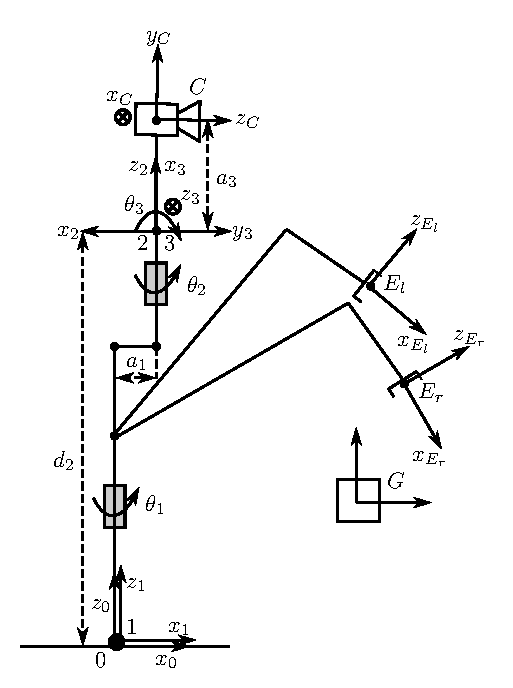
\includegraphics[trim=0.0cm 0.1cm 0.0cm 0.0cm, clip=true, width=0.95\linewidth]{./Img/velma_b_v2.pdf}
		\end{center}
        \caption{Example}
        \label{fig:qqq}
    \end{figure}

    
	\section{Conclusions}
	\label{sec:Conclusions}
	\hl{Nie uzupelniac}
	
	\bibliographystyle{spmpsci}
	\bibliography{references}
	
	\section*{Statements and Declarations}
	
	The authors declare that no funds, grants, or other support were received during the preparation of this manuscript.
	
	The authors have no relevant financial or non-financial interests to disclose.
		
	The datasets generated during and/or analyzed during the current study are not publicly available due to complexity of the experiments, but are available from the corresponding author on reasonable request.
	
\end{document}




